\section{可积函数的逼近}
\label{sec:fapprox-integrable}

有限维中有一个基本事实：有理分量的向量在$\mathbb R^n$中稠密，任何向量都能被它们以任意精度接近。可积函数这种“无限长的向量”可能处处不连续，也可能无界，我们希望知道它能否被结构简单的函数接近。这样，许多论证就可以先对简单函数验证，再推广到一般函数。

用第~\ref{chap:topological-spaces}章的语言，这是在问某个函数族在$L^p$中是否稠密，能否取到可数的稠密族。第~\ref{chap:metric-spaces}章的距离和点列判据，把问题化为构造一列误差趋于零的近似。本节依次使用简单函数、连续函数和光滑函数，每一步都核对所用的测度、指数$p$与范数。

\subsection{简单函数逼近}
\label{sec:fapprox-simple}

只取有限多个值的可测函数称为简单函数，可以写成
\[
 s=\sum_{i=1}^kc_i\mathbf 1_{A_i},\qquad A_i\ \text{可测},\quad c_i\in\mathbb K .
\]
用向量的话说，这是分量只有有限种不同取值的向量，就像把一个长向量的每个分量四舍五入到有限个档位。第~\ref{chap:measure}章已经用取值分层构造了逐点收敛的简单函数列，这里要问的是：误差用$L^p$范数衡量时，它是否也趋于零。

\paragraph{截断与取值分层}
对非负函数，把取值范围按二进分层，每层取下端点，再把过大的值截断。设$f\geq0$可测，令
\begin{equation}
 s_n=\min\bigl\{n,\ 2^{-n}\lfloor2^nf\rfloor\bigr\},\qquad n=1,2,\ldots .
 \label{eq:fapprox-dyadic-simple}
\end{equation}
这里做了两件事：$\lfloor2^nf\rfloor/2^n$相当于把分量舍入到间距为$2^{-n}$的档位，取$\min$相当于把超过$n$的大分量压到$n$。

在$f$落入$[j2^{-n},(j+1)2^{-n})$的集合上，$s_n$取值$j2^{-n}$；在$f\geq n$的集合上，$s_n$取值$n$。所以$s_n$只取有限多个值。同时，每一点都有
\[
 0\leq s_n\leq f,
\]
并且在$f<n$处有
\[
 0\leq f-s_n<2^{-n}.
\]
$f$有限的点上，$n$足够大后都落在第二种情形，所以$s_n\to f$逐点成立。

\begin{theorem}[简单函数逼近$L^p$函数]
\label{thm:fapprox-simple-dense}
设$(X,\mathcal A,\mu)$为测度空间，$1\leq p<\infty$，$f\in L^p(\mu)$。则存在一列简单函数$s_n=\sum_ic_{n,i}\mathbf 1_{A_{n,i}}$，其中每个$\mu(A_{n,i})<\infty$，使$\lVert f-s_n\rVert_p\to0$。
\end{theorem}

\begin{proof}
先设$f\geq0$，取式~\eqref{eq:fapprox-dyadic-simple}中的$s_n$。$f\in L^p$说明$f$几乎处处有限，于是$\lvert f-s_n\rvert^p\to0$几乎处处成立。又由$0\leq s_n\leq f$，
\[
 \lvert f-s_n\rvert^p\leq f^p ,
\]
右端可积，控制收敛定理给出$\lVert f-s_n\rVert_p\to0$。

再看取值集合的测度。$n\geq1$时，$s_n$的非零取值都不小于$2^{-n}$，所以$\{s_n\neq0\}\subseteq\{f\geq2^{-n}\}$。由Chebyshev不等式，
\[
 \mu(\{s_n\neq0\})\leq\mu(\{f\geq2^{-n}\})\leq2^{np}\lVert f\rVert_p^p<\infty ,
\]
每个非零取值所在的集合测度都有限。

一般的实值$f$写成$f=f^+-f^-$，复值$f$再分实部与虚部。每一部分分别按上面逼近，组合后的误差由三角不等式控制，取值集合仍测度有限。
\end{proof}

这里$p<\infty$用了两次：控制收敛需要$f^p$可积，有限测度的支撑来自Chebyshev不等式。结论只说明简单函数在$L^p(\mu)$中稠密，并没有给出可数的稠密族，因为可测集$A_{n,i}$可以有不可数多种选法。

\begin{example}[两部分误差的大小]
取$(0,1]$上的$f(x)=x^{-1/3}$，$p=2$。它无界，但$\int_0^1x^{-2/3}\,\mathrm dx=3$，所以$f\in L^2$。我们把误差分成被截断的部分和分层舍入的部分分别计算。

$f\geq n$等价于$x\leq n^{-3}$。在这一段上$s_n=n$，平方误差是
\[
 \int_0^{n^{-3}}\bigl(x^{-1/3}-n\bigr)^2\,\mathrm dx
 =\Bigl[3x^{1/3}-3nx^{2/3}+n^2x\Bigr]_0^{n^{-3}}.
\]
代入上限，三项依次是$3/n$、$-3/n$、$1/n$，所以
\[
 \int_0^{n^{-3}}\bigl(x^{-1/3}-n\bigr)^2\,\mathrm dx=\frac1n .
\]

在其余部分，逐点误差小于$2^{-n}$，区间长度不超过$1$，平方误差不超过$4^{-n}$。合起来，
\[
 \lVert f-s_n\rVert_2^2\leq\frac1n+4^{-n}.
\]
$n=2$时右端是$0.5+0.0625$，$n=10$时约为$0.1$。舍入误差按指数下降，真正慢的是截断带来的误差。

若把$p=2$换成$p=3$，则$\int_0^1x^{-1}\,\mathrm dx=\infty$，$f$不属于$L^3$，定理不适用。此时被截断部分的三次积分也发散，误差始终是无穷大。
\end{example}

\paragraph{Lebesgue区域上的可数逼近族}
$\mathbb R^n$中用有理分量得到可数稠密集。在欧氏空间的函数上，同样的想法分两步：可测集用矩形逼近，矩形和系数都只取有理数。设$\Omega\subseteq\mathbb R^d$可测，取Lebesgue测度$\lambda$。称各边端点都是有理数的矩形$R=\prod_{i=1}^d[a_i,b_i)$为有理矩形，令$\mathcal D$为全体有限和
\[
 \sum_{i=1}^kc_i\mathbf 1_{R_i\cap\Omega},\qquad R_i\ \text{为有理矩形},\quad \operatorname{Re}c_i,\operatorname{Im}c_i\in\mathbb Q .
\]
有理矩形只有可数多个，系数也只有可数多种，所以$\mathcal D$可数。

\begin{theorem}[$L^p(\Omega)$的可数稠密族]
\label{thm:fapprox-separable}
在上述记号下，设$1\leq p<\infty$，则$\mathcal D$在$L^p(\Omega)$中稠密，因而$L^p(\Omega)$可分。
\end{theorem}

\begin{proof}
先化简目标。由定理~\ref{thm:fapprox-simple-dense}和三角不等式，只需逼近有限测度可测集$A\subseteq\Omega$的示性函数，系数换成有理复数只带来任意小的误差。对有理矩形的有限并$U$，有
\[
 \lVert\mathbf 1_A-\mathbf 1_{U\cap\Omega}\rVert_p^p=\lambda\bigl(A\mathbin{\triangle}(U\cap\Omega)\bigr)\leq\lambda(A\mathbin{\triangle}U),
\]
所以只需对任意$\varepsilon>0$，找到$U$使$\lambda(A\mathbin{\triangle}U)$小于$3\varepsilon$。

第一步，用可数个矩形覆盖$A$。由Lebesgue测度的定义（第~\ref{chap:measure}章），存在矩形$R_1,R_2,\ldots$覆盖$A$，并且$\sum_i\lambda(R_i)<\lambda(A)+\varepsilon$。于是
\[
 \lambda\Bigl(\bigcup_iR_i\setminus A\Bigr)<\varepsilon .
\]

第二步，截成有限个。级数收敛，取$N$使$\sum_{i>N}\lambda(R_i)<\varepsilon$，令$U_0=\bigcup_{i\leq N}R_i$。由$A\setminus U_0\subseteq\bigcup_{i>N}R_i$，$\lambda(A\setminus U_0)<\varepsilon$。又$U_0\setminus A\subseteq\bigcup_iR_i\setminus A$，合起来
\[
 \lambda(A\mathbin{\triangle}U_0)<2\varepsilon .
\]

第三步，把端点换成有理数。把每个$R_i$（$i\leq N$）放大成有理矩形$R_i'\supseteq R_i$，使$\lambda(R_i'\setminus R_i)<\varepsilon/N$，这只需把各端点向外移到足够近的有理数。令$U=\bigcup_{i\leq N}R_i'$，则$\lambda(U\setminus U_0)<\varepsilon$，所以
\[
 \lambda(A\mathbin{\triangle}U)<3\varepsilon .
\]
最后，有限个有理矩形的并可以用所有端点坐标切成有限个两两不交的有理矩形，因此$\mathbf 1_{U\cap\Omega}$属于$\mathcal D$。
\end{proof}

\paragraph{一般测度空间的条件}
上面的证明只用到一点：存在可数个有限测度集组成的族，使每个有限测度可测集都能用其中有限个的并按测度逼近。一般测度空间中这需要另外核对。

反例是不可数集$I$上的计数测度，此时$L^p$就是$\ell^p(I)$。这个“向量”有不可数个分量，单点示性函数$\mathbf 1_{\{i\}}$是坐标向量，两两距离为$2^{1/p}$。以它们为中心、半径$2^{1/p}/2$的开球两两不交且有不可数个，而稠密子集必须在每个球中都有元素，所以不存在可数稠密子集。

\paragraph{有界函数与本质上确界}
$p=\infty$时情况又不同。$L^\infty$范数相当于取向量各分量绝对值的最大值，这把尺子不允许任何一段上的误差被平均掉。在$L^\infty[0,1]$中取$f_t=\mathbf 1_{[0,t]}$，$0<t<1$。对$s<t$，差$f_t-f_s=\mathbf 1_{(s,t]}$在正测度集上等于$1$，所以
\[
 \lVert f_t-f_s\rVert_\infty=1 .
\]
半径$1/2$的球$\{g:\lVert g-f_t\rVert_\infty<1/2\}$两两不交，共有不可数个，同样的论证说明$L^\infty[0,1]$没有可数稠密子集。

但简单函数在$L^\infty$中仍然稠密。设$f$是实值本质有界函数，取一个满足$\lvert f\rvert\leq M$处处成立的代表。取$n\geq M$，对$f^+$与$f^-$分别作式~\eqref{eq:fapprox-dyadic-simple}的分层，组合后得到$s_n$，于是
\[
 \lVert f-s_n\rVert_\infty\leq2^{-n}.
\]
复值时分实部与虚部处理。

这两个结论并不矛盾。这里的简单函数，其取值集合是$f$的水平集，可以有不可数多种，无法取成可数族；可数的有理矩形虽然能按测度逼近这些集合，却控制不了本质上确界：把集合修改一小块，$L^\infty$误差仍可能是$1$。

\subsection{光滑函数逼近}
\label{sec:fapprox-smooth}

简单函数一般不连续。许多论证希望先对连续甚至光滑的函数推导，例如把导数移到另一个函数上，再推广到一般函数。本小节在欧氏开集$\Omega\subseteq\mathbb R^d$上取Lebesgue测度，分三步建立这种逼近：先用集合的开紧逼近得到连续函数，再证明平移在$L^p$中连续，最后用第~\ref{chap:smoothing-weak-derivatives}章的卷积磨光得到光滑函数。

\paragraph{紧支撑连续函数}
记$C_c(\Omega)$为$\Omega$上支撑为紧集的连续函数。第~\ref{chap:smoothing-weak-derivatives}章由矩形覆盖推出了Lebesgue测度的正则性：对有限测度可测集$A\subseteq\Omega$和$\varepsilon>0$，存在紧集$K$与开集$U$，使$K\subseteq A\subseteq U\subseteq\Omega$且$\lambda(U\setminus K)<\varepsilon$。于是示性函数$\mathbf 1_A$的棱角可以夹在$K$与$U$之间用一个连续的“斜坡”磨掉。

\begin{theorem}[紧支撑连续函数逼近$L^p$函数]
\label{thm:fapprox-cc-dense}
设$\Omega\subseteq\mathbb R^d$为开集，$1\leq p<\infty$，则$C_c(\Omega)$在$L^p(\Omega)$中稠密。
\end{theorem}

\begin{proof}
由定理~\ref{thm:fapprox-simple-dense}，只需逼近有限测度集$A\subseteq\Omega$的示性函数。按上面的正则性取$K\subseteq A\subseteq U$，$\lambda(U\setminus K)<\varepsilon$。若$K$是空集，取$\varphi=0$，此时误差的$p$次方不超过$\lambda(U)<\varepsilon$。下设$K$非空。

为使连续函数有紧支撑，先把$U$缩小。$K$紧且含于开集$\Omega$，它到$\Omega$的补集有正距离（$\Omega=\mathbb R^d$时这一距离取为$+\infty$）。取$\delta>0$小于这个距离，令
\[
 U'=U\cap\{x:\operatorname{dist}(x,K)<\delta\}.
\]
$U'$仍是包含$K$的开集，它的闭包含于有界闭集
\[
 \{x:\operatorname{dist}(x,K)\leq\delta\}\subseteq\Omega ,
\]
因而是$\Omega$内的紧集。

定义斜坡函数
\[
 \varphi(x)=\frac{\operatorname{dist}(x,U'^c)}{\operatorname{dist}(x,U'^c)+\operatorname{dist}(x,K)} .
\]
$K$与闭集$U'^c$不交，分母处处为正，所以$\varphi$连续。它在$K$上等于$1$，在$U'$外等于$0$，取值在$[0,1]$中，支撑含于$U'$的闭包，因而$\varphi\in C_c(\Omega)$。

最后估计误差。$\mathbf 1_A$与$\varphi$在$K$上都等于$1$，在$U$外都等于$0$，所以$\mathbf 1_A-\varphi$只在$U\setminus K$上可能非零，并且绝对值不超过$1$。于是
\[
 \lVert\mathbf 1_A-\varphi\rVert_p^p\leq\lambda(U\setminus K)<\varepsilon .
\]
\end{proof}

\paragraph{平移的$L^p$连续性}
磨光是对附近的平移作平均，所以要先知道小平移在$L^p$范数下改变函数多少。对长向量来说，平移就是把所有分量的下标错开一位。记$(\tau_hf)(x)=f(x-h)$。Lebesgue测度在平移下不变，所以$\lVert\tau_hf\rVert_p=\lVert f\rVert_p$。第~\ref{chap:smoothing-weak-derivatives}章对$p=1$证明了平移的积分连续性，下面对一般有限$p$给出同样的结论。

\begin{theorem}[平移在$L^p$中连续]
\label{thm:fapprox-translation}
设$1\leq p<\infty$，$f\in L^p(\mathbb R^d)$，则$\lVert\tau_hf-f\rVert_p\to0$（$h\to0$）。
\end{theorem}

\begin{proof}
先设$g\in C_c(\mathbb R^d)$，支撑含于球$B_R$。$g$一致连续，记
\[
 \omega_g(t)=\sup_{\lvert x-y\rvert\leq t}\lvert g(x)-g(y)\rvert ,
\]
则$\omega_g(t)\to0$。对$\lvert h\rvert\leq1$，$\tau_hg-g$的支撑含于$B_{R+1}$，所以
\[
 \lVert\tau_hg-g\rVert_p^p\leq\omega_g(\lvert h\rvert)^p\,\lambda(B_{R+1})\to0 .
\]

一般地，任给$\varepsilon>0$，由定理~\ref{thm:fapprox-cc-dense}取$g\in C_c(\mathbb R^d)$使$\lVert f-g\rVert_p<\varepsilon$。三角不等式把$\tau_hf-f$分成三段：
\[
 \lVert\tau_hf-f\rVert_p\leq\lVert\tau_h(f-g)\rVert_p+\lVert\tau_hg-g\rVert_p+\lVert g-f\rVert_p .
\]
由平移不变性，第一项等于$\lVert f-g\rVert_p<\varepsilon$；第三项也小于$\varepsilon$。于是
\[
 \lVert\tau_hf-f\rVert_p<2\varepsilon+\lVert\tau_hg-g\rVert_p ,
\]
最后一项在$h$充分小时小于$\varepsilon$。
\end{proof}

$p=\infty$时结论不成立。在$\mathbb R$上取$f=\mathbf 1_{[0,1/2]}$。对$0<\lvert h\rvert<1/2$，$\tau_hf-f$在两个长为$\lvert h\rvert$的区间上取值$\pm1$，所以
\[
 \lVert\tau_hf-f\rVert_\infty=1 .
\]
积分范数允许误差集中在测度很小的集合上，本质上确界不允许。

\paragraph{磨光的$L^p$收敛}
取第~\ref{chap:smoothing-weak-derivatives}章的磨光核：$\rho$光滑、非负、积分为$1$、支撑于单位闭球，缩放后记为
\[
 \rho_\varepsilon(x)=\varepsilon^{-d}\rho(x/\varepsilon).
\]
那里证明了$f_\varepsilon=\rho_\varepsilon*f$光滑，并在$L^1$意义下局部逼近$f$。用向量的话说，$f_\varepsilon$是对相邻分量做加权滑动平均；下面在全空间上证明$L^p$收敛，误差由平移误差控制。

\begin{theorem}[磨光在$L^p$中收敛]
\label{thm:fapprox-mollifier}
设$1\leq p<\infty$，$f\in L^p(\mathbb R^d)$，$f_\varepsilon=\rho_\varepsilon*f$。则
\begin{equation}
 \lVert f_\varepsilon-f\rVert_p\leq\sup_{\lvert h\rvert\leq\varepsilon}\lVert\tau_hf-f\rVert_p\to0\qquad(\varepsilon\to0).
 \label{eq:fapprox-mollifier-error}
\end{equation}
\end{theorem}

\begin{proof}
由$\int\rho_\varepsilon=1$，可以把$f(x)$写进平均里：
\[
 f_\varepsilon(x)-f(x)=\int\rho_\varepsilon(h)\bigl(f(x-h)-f(x)\bigr)\,\mathrm dh .
\]

$p>1$时记$q=p/(p-1)$，把被积函数写成$\rho_\varepsilon^{1/q}\cdot\rho_\varepsilon^{1/p}\lvert f(x-h)-f(x)\rvert$。由Hölder不等式与$\int\rho_\varepsilon=1$，
\[
 \lvert f_\varepsilon(x)-f(x)\rvert^p\leq\int\rho_\varepsilon(h)\,\lvert f(x-h)-f(x)\rvert^p\,\mathrm dh .
\]
$p=1$时这就是绝对值不等式。

被积函数非负可测，对$x$积分并由Tonelli定理交换积分次序，
\[
 \lVert f_\varepsilon-f\rVert_p^p\leq\int\rho_\varepsilon(h)\,\lVert\tau_hf-f\rVert_p^p\,\mathrm dh .
\]
$\rho_\varepsilon$支撑于半径$\varepsilon$的闭球且积分为$1$，所以右端是$\lVert\tau_hf-f\rVert_p^p$的加权平均，不超过它在$\lvert h\rvert\leq\varepsilon$上的上确界。由定理~\ref{thm:fapprox-translation}，这一上确界随$\varepsilon\to0$趋于零。
\end{proof}

跳跃函数最能说明指数$p$的作用。取$\mathbb R$上的$f=\mathbf 1_{[0,1/2]}$，当$\varepsilon\leq1/4$时，$f_\varepsilon-f$只集中在两个跳跃点两侧宽$\varepsilon$的带内。记$T(u)=\int_u^1\rho(v)\,\mathrm dv$，代换$x=\varepsilon u$后，两个跳跃点各贡献两段相同的积分，得到
\[
 \lVert f_\varepsilon-f\rVert_p^p=4\varepsilon\int_0^1T(u)^p\,\mathrm du .
\]

所以$L^p$误差按$\varepsilon^{1/p}$下降：$p=1$时是一阶，$p=2$时是$\varepsilon^{1/2}$。$p$越大，指数$1/p$越小。到$p=\infty$，指数变成零，而跳跃点处$f_\varepsilon$的值恒为$1/2$，误差$1/2$不再变化。图~\ref{fig:fapprox-mollifier-norms}把这件事画了出来：曲线明显向跳跃靠拢，$L^1$与$L^2$的误差都在下降，一致误差却保持不动。

\begin{BookInlineFigure}
  \centering
  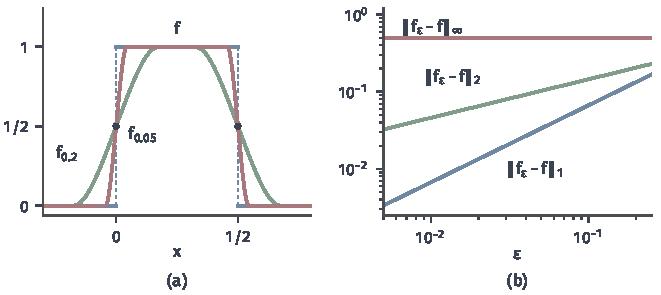
\includegraphics[width=112mm]{figures/04-spaces-measures-and-geometry/03-function-spaces/matplotlib/fapprox-mollifier-norms/figure.pdf}
  \caption{跳跃函数的磨光。(a)$f=\mathbf 1_{[0,1/2]}$（蓝）与$\varepsilon=0.2$（绿）、$\varepsilon=0.05$（红）的磨光；两个黑点标出无论$\varepsilon$多小，$f_\varepsilon$在跳跃点都等于$1/2$。(b)三种范数下的误差随$\varepsilon$的变化，双对数坐标：$L^1$误差为$2m_1\varepsilon$（$m_1\approx0.3345$），$L^2$误差正比于$\varepsilon^{1/2}$，$L^\infty$误差恒为$1/2$。}
  \label{fig:fapprox-mollifier-norms}
\end{BookInlineFigure}

\paragraph{光滑紧支撑函数与局部逼近}
两步合起来就得到光滑函数的逼近。设$f\in L^p(\Omega)$，$1\leq p<\infty$，$\varepsilon_0>0$。由定理~\ref{thm:fapprox-cc-dense}取$g\in C_c(\Omega)$使$\lVert f-g\rVert_p<\varepsilon_0$，把$g$在$\Omega$外延拓为零。

$\rho_\varepsilon*g$光滑，支撑含于$\operatorname{supp}g$的$\varepsilon$邻域。取$\varepsilon$小于$\operatorname{supp}g$到$\Omega^c$的距离，它就属于$C_c^\infty(\Omega)$。由定理~\ref{thm:fapprox-mollifier}，再取$\varepsilon$足够小，使$\lVert\rho_\varepsilon*g-g\rVert_p<\varepsilon_0$。所以$C_c^\infty(\Omega)$在$L^p(\Omega)$（$1\leq p<\infty$）中稠密。

只在局部可积的函数也有局部版本，办法是先截断。设$f\in L^p_{\mathrm{loc}}(\Omega)$，即在每个紧集上$p$次可积，$K\subset\Omega$紧。取$\delta>0$使闭邻域
\[
 K_\delta=\{x:\operatorname{dist}(x,K)\leq\delta\}
\]
含于$\Omega$，令$F=f\mathbf 1_{K_\delta}$，则$F\in L^p(\mathbb R^d)$。

对$\varepsilon<\delta$和$x\in K$，$\rho_\varepsilon(x-\cdot)$的支撑落在$K_\delta$内，所以$(\rho_\varepsilon*F)(x)=f_\varepsilon(x)$。由定理~\ref{thm:fapprox-mollifier}，
\[
 \int_K\lvert f_\varepsilon-f\rvert^p\,\mathrm dx\leq\lVert\rho_\varepsilon*F-F\rVert_p^p\to0 .
\]
截断把局部问题化为全空间问题，代价是结论只在远离边界的紧集上成立。

\paragraph{$L^\infty$中的失效}
连续函数在$L^\infty$中不稠密，光滑函数更是如此。在$(0,1)$上取$f=\mathbf 1_{(0,1/2]}$。设$g$连续且$\lVert g-f\rVert_\infty=r$，则下面两个不等式都几乎处处成立：
\[
 g\geq1-r\ \text{在}\ (0,1/2)\ \text{上},\qquad g\leq r\ \text{在}\ (1/2,1)\ \text{上}.
\]
满测度集在区间中稠密，由连续性这两个不等式在相应闭区间上处处成立。取$x=1/2$，得到
\[
 1-r\leq g(1/2)\leq r ,
\]
即$r\geq1/2$。所以任何连续函数与$f$的本质上确界距离都不小于$1/2$，这正是跳跃幅度的一半。

本节的结论都是定性的：对每个精度都存在某个近似，但没有说明近似需要多少参数。简单函数要多少层、磨光宽度要多小，取决于目标函数本身，而定理没有给出任何速率。要比较不同表示的效率，必须先固定允许使用多少参数，这是下一节的任务。
